
% SECTION:
%    transient.tex  
%
% CHAPTER:
%    transients.tex  
%
% ELEVATOR PITCH:
%    Explain in a few sentences what the relevant discovery or
%    measurement is going to be discussed, and what will be important
%    about it. This is for the browsing reader to get a quick feel
%    for what this section is about.
%
% COMMENTS:
%
%
% BUGS:
%
%
% AUTHORS:
%  Stefano Valenti , Federica Bianco (@fedhere)
%
% ====================================================================

\section{Young Transients Discrimination Power}
\def\secname{transientsAge}\label{sec:\secname} % For example, replace "keyword" with "lenstimedelays"

\credit{svalenti}\credit{fedhere} % (Writing team)

In this section we investigate the identification of young transients using the intra-night visits. The Baseline Cadence~\opsimdbref{db:baseCadence} predicts that, on average, fields in the main survey are revisited every $\sim3$ days in any filter (Figure~\ref{fig:enigmaGapAll}), and every $\sim15$ days when using only $r$ band visits (Figure~\ref{fig:enigmaGapr}).  Hence, we are likely to discover transients when they are between 0 and 3 days old. However, for many transients it is the first few hours after event beginning that reveal fundamental information on the nature of transients. Since real time discrimination is a very hard task, it is then important to be able to select, among the large number of transients discovered by LSST, the youngest objects, in order to device follow-up plans, and best distribute follow-up resources. Within the~\opsimdbref{db:baseCadence} cadence, and most cadences realized thus far, the second intra-night visit should occur between 30 minutes to 2 hours after the first visit (to maximize the Solar System moving objects recovery,~\ref{chp:solarsystem}). We want to understand how the {\bf\emph{intra-night gap enables, affects, and maximizes the identification of new transients as young (i.e. within a day of outburst/explosion.}}
To begin to answer this question, we limit our investigation to lightcurve shape alone, and specifically to what can be done in $r$ band. We have selected a representative set of transients with good photometric coverage in the first week after the the outburst/explosion (see left panel of Figure~\ref{fig:earlyslope}) and computed the light curve slope as a function of time in magnitudes per day (right panel of Figure~\ref{fig:earlyslope})). In Figure~\ref{fig:earlyrise} we report the change in $r$ brightness between the first and the second visit for the same set of transients as function of phase.

Despite the heterogeneity in light curve shapes most of the transients show a similar change in brightenss on short time scales. 
This confirms that early classification and identification of interesting transients in real time is a major challenge. However, independently on the type of transient, although in general new transients have a large increase in brightnessit, is much easier to assess wheather a transients is \emph{young} with large time gap between visits (e.g. 2 hours).
Within 30 minutes the change in brightness is of the order of $1\%$, or even less, for most transients that we investigated within the first $\sim3$ days from the start of the outburst/explosion (Figure~\ref{fig:earlyslope}, left). Thus a measurement of the change would require a $SNR\gtrsim500$ on each measurement. With a time gap of $\sim2$~hours after the first visit, the change of brightness will increase to $\sim5\%$. However the breadth of the gap is not of course unlimited: a gap of even 24 hours, while helpful in identifying young transients, does not by itself enable identification of the type of transient.  The identification of interesting transients, at an early stage, can be aided by using supplementary information, such as historical information from previous visits or color information about the transient. But to properly assess the color of an evolving transient, the observation pair has to be simultaneous, or separated by a small gap~\ref{sec:SNtransients}.

Finally, we stress that the quality and copleteness of early multiwavelengh data available at this time is limited; the sample of astronomical transients used here is not comprehensive and a uniform set of homogeneous data of different transients is still needed in order to further investigate the ideal separation between observations, the need for color information, and the tension between the two. 

\begin{figure}[hbt]
\centerline{
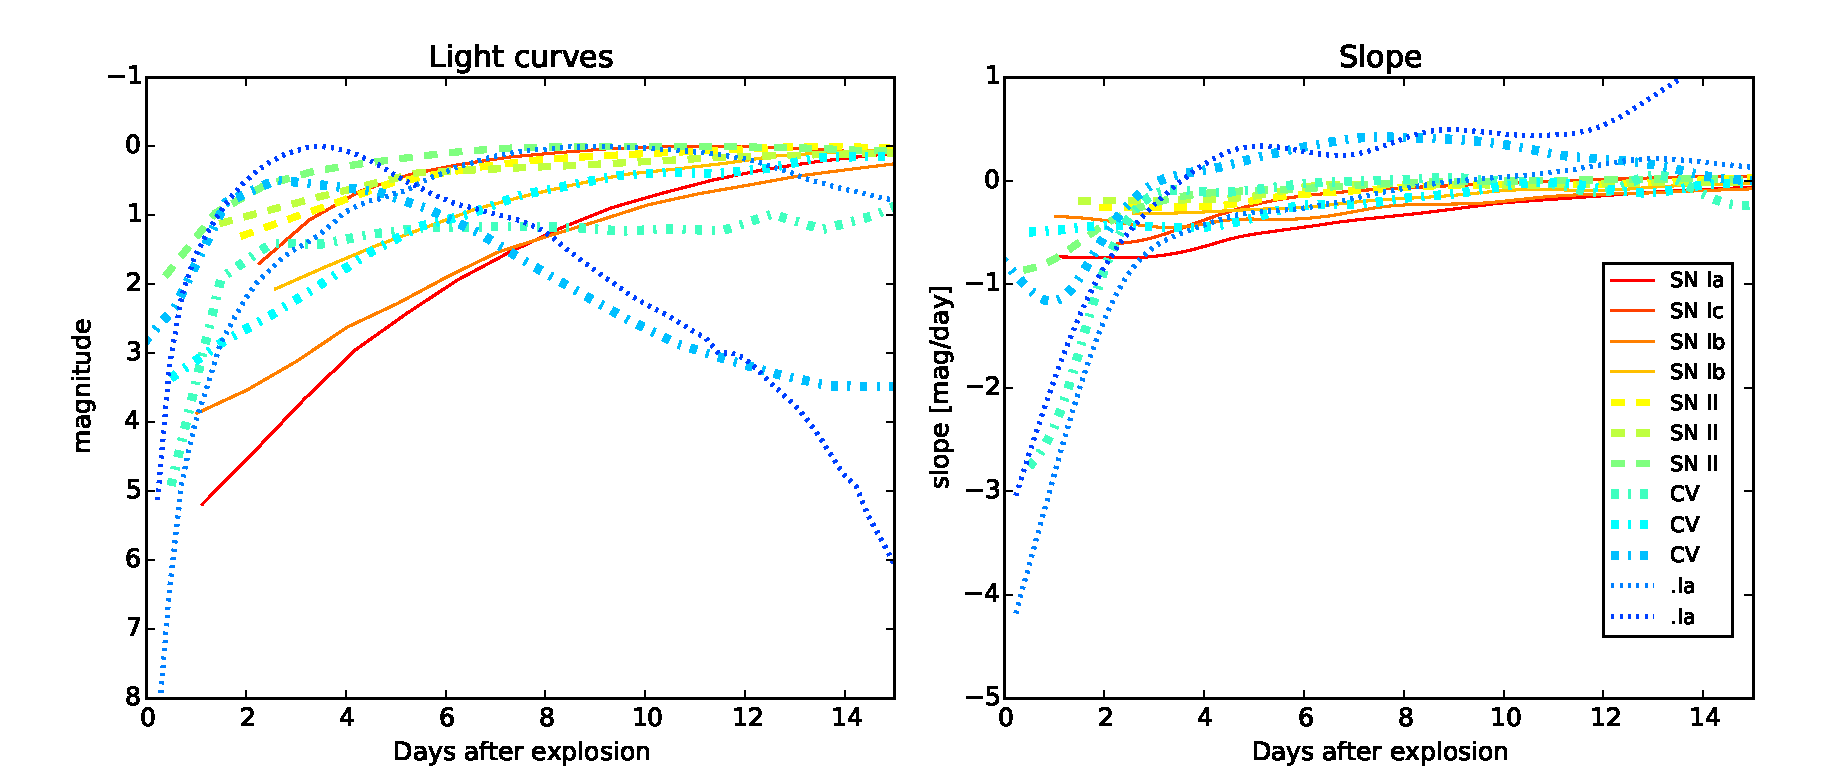
\includegraphics[width=0.6\textwidth]{figs/transients/earlyslope.pdf}
}
\caption{\emph{Left}: $r'$-band light curve for representative transients as function of the phase from the beginning of the transient outburst/explosion for the first few days of the transient life. \emph{Right}: slope of the transient evolution. Data from: SN~Ia,~\citet{Olling15}; SNII,~\citet{Rubin16}; SN~.Ia,~\citet{Shen10}; SN~Ib,~\citet{Valenti11},~\citet{Cao13}; SN~Ic,~\citet{Mazzali02}; CV, ~\citet{Sokoloski13}, Finzell et al. (in prep).}
\label{fig:earlyslope}
\end{figure}

\begin{figure}[hbt]
\centerline{
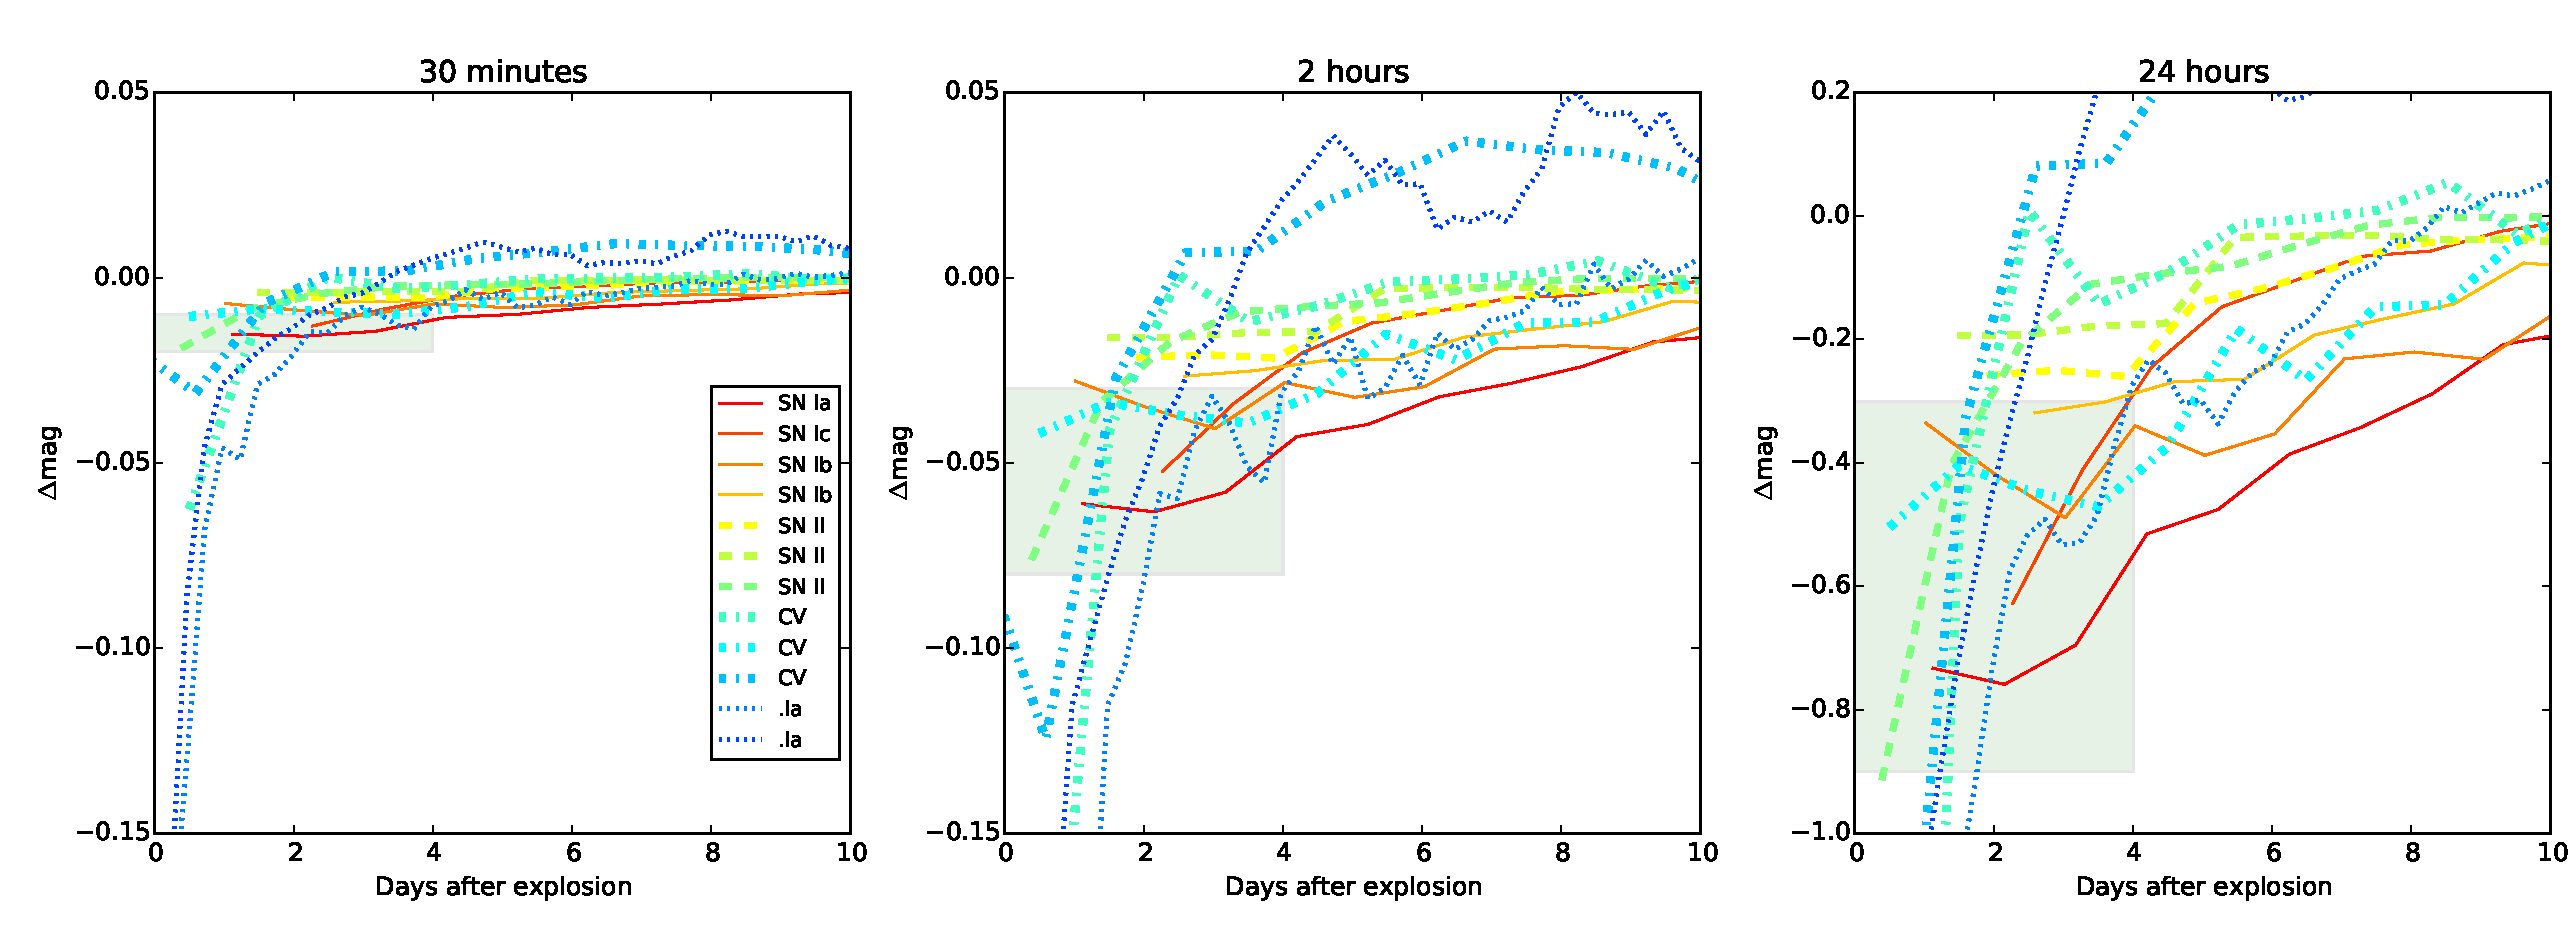
\includegraphics[width=0.6\textwidth]{figs/transients/earlyrise.pdf}
}
\caption{Observed magnitude change between two consecutive observations for a representative set of astronomical transients, as a function of the phase. We consider observation gaps of 30 minutes  (left panel), 2 hours (central panel) and 24 hours (right panel). 
}
\label{fig:earlyrise}
\end{figure}
